\documentclass{article}
\usepackage[14pt]{extsizes}
\linespread{1.3}
\usepackage[T2A]{fontenc}
\usepackage[utf8x]{inputenc}
\usepackage[english,russian]{babel}
\usepackage{listings}
\usepackage{graphicx}
\usepackage[left=3cm,right=1cm,top=2cm,bottom=2cm,bindingoffset=0cm]{geometry}
\righthyphenmin=2


\begin{document}
\begin{titlepage}

\begin{center}
\bf Министерство образования и науки Российской Федерации
Московский физико-технический институт
 ( государственный университет )
\vspace{1cm}
Факультет радиотехники и кибернетики
Кафедра информатики и вычислительной техники
\vspace{3cm}
\end{center}
\begin{flushright}
\vbox{
На правах рукописи\\
УДК 004.454
}
\end{flushright}

\vspace{4em}

\begin{center}
Демидов Арсений Александрович\\
\large Реализация состояния глубокого сна микропроцессора Эльбрус-4С при помощи средств ядра Linux\\
\vspace{1.5em}
\large{Выпускная квалификационная  работа бакалавра}
\end{center}
\vspace{1.5em}
\begin{center}
 Направление подготовки 010900: Прикладные математика и физика
\end{center}
\vspace{7em}

\begin{flushleft}
Заведующий кафедрой д.т.н. проф. Перекатов В. И. \\
Научный руководитель д.т.н. проф. Кравцунов Е. \\
Студент Демидов А. А. \\
\end{flushleft}

\vfill

\begin{center}
г.Москва
2017
\end{center}

\end{titlepage}


\tableofcontents
\setcounter{page}{2}
\newpage

\section{Введение}

Одной из наиболее значимых проблем, стоящих в настоящее время перед производителями и пользователями вычислительных средств, является управление энергопотреблением. Так, плата за энергопотребление мощных серверов, входящих в состав высокопроизводительных вычислительных комплексов (ВК), стала основой затрат на их обслуживание, а в категории мобильных и встраиваемых систем эффективное управление энергопотреблением позволяет улучшить одну из главных характеристик --- максимальное время функционирования в автономном режиме (от батареи). В компании ЗАО «МЦСТ» исследования и разработки, связанные с этой проблемой, начались в 2011 г. в связи с проектированием процессоров для мобильных систем.

В данной работе, построенной на основе проведенных ранее исследований по части
поддержки стандарта ACPI в архитектуре Эльбрус описывается набор состояний С0,С1,С3, реализация состояния С3 для микропроцессоров Эльбрус--4С и Эльбрус--8С и подробно изучена энергосберегающая подсистема ядра Linux --- cpuidle.

Система работает под управлением ОС Linux-2.6.33, в ядре которой присутствует
архитектурно-независимая реализация алгоритмов управления энергосбережением, разработанная силами Linux сообщества.

Тестирование проводилось на вычислительных комплексах на базе микропроцессоров Эльбрус--8С и Эльбрус--4С.

\subsection{Цель работы}
Целью данной работы является снижение энергопотребления ВК на базе микропроцессоров Эльбрус--4С и Эльбрус--8С во время простоя (idle)
\subsection{Задачи}
Для достижения поставленной цели решались следующие задачи:
\begin{itemize}
\item Реализация функциональности перевода вычислительного ядра в состояние глубокого сна
\item Реализация в составе подсистемы cpuidle
\end{itemize}
\subsection{Требования}
Возможность управления через интерфейс sysfs


\newpage
\section{Состояния ядер микропроцессора}

Общепринятый подход к снижению уровня энергопотребления сформулирован в стандарте ACPI \cite{acpi}, который в ряде распространенных архитектур поддерживается на аппаратном уровне. Согласно этому стандарту для ВК определяется несколько наборов состояния энергосбережения. Наиболее общим является набор {S0;Sn}, характеризующий энергосберегающие состояния ВК в целом с учетом процессоров, памяти, шин, периферийных устройств. Любое состояние Si из этого набора определяется тремя значениями (Ci, Pi, Di), каждое из которых принадлежит одному из трех наборов состояний, соответственно {C0;Cn}, {P0;Pn} и {D0;Dn}. Здесь {С0;Сn} – набор состояний сна для процессорного ядра, {P0;Pn} – набор активных состояний с различной частотой для процессорного ядра, {D0;Dn} – набор энергосберегающих состояний шин, памяти, контроллеров ввода вывода и периферийных устройств, расположенных на материнской плате. В соответствии со стандартом, переходы из одного состояния в другое инициируются операционной системой. 

\subsection{Состояния сна}

Как было сказано выше стандарт ACPI включает в себя состояния C0, C1, C2, ... , Cn. Где С0 активное состояние при котором центральный процессор выполняет инструкции. Состояния с С1 по Cn это состояния сна потребляющие меньше энергии и рассеивающие меньше тепла. В состоянии сна процессор не выполняет никаких инструкций. Каждое состояние сна имеет задержку, связанную с входом и выходом из этого состояния, что способствует экономии электроэнергии. В целом, чем дольше задержка ввода/вывода, тем больше экономия электроэнергии в этом состоянии. Для экономии электроэнергии, операционная система размещает ЦП в одно из поддерживаемых состояний во время простоя.

Выделяют три состояния функционирования ядер микропроцессоров семейства Эльбрус\cite{kravc1,kravc2}
\begin{itemize}
\item С0 – оперативный режим
\item С1 – отключение конвейера
\item С3 – гашения кэш-памятей и отключение синхросигнала (глубокий сон)
\end{itemize}

Возврат из состояний С1 и С3 происходит при поступлении на контроллер прерываний ядра (lapic) внешнего прерывания. Времена возврата в состояние C0 различны для разных состояний сна --- так, время возврата из C1 существенно меньше времени возврата из C3

Следует отметить, что в ядре ОС Эльбрус нет реализации перехода в состояние С3.


\newpage
\section{Перевод вычислительного ядра в С3 }

\subsection{Описание алгоритма}

Фрагмент кода, приводящий к выключению синхронизации вычислительного ядра,
должен соответствовать нижеперечисленным правилам, иначе возможна подмена данных
или "зависание" ядра или даже всей машины.
\begin{enumerate}

\item Код выключения ядра должен быть резидентным как в физической, так и в виртуальной памяти.

\item Код выключения ядра должен быть немодифицируемым.

\item Код выключения ядра исполняется на том же ядре.

\item Код выключения ядра не должен содержать операций обращения в память, за
исключением приведенных ниже спецопераций.

\item Код выключения ядра не должен содержать операций подготовки перехода и
предподкачки кода.

\item Код выключения ядра должен содержать инвалидацию регистров подготовки
перехода. Это позволяет избежать слабоконтролируемых спекулятивных обращений в
память от незавершенных операций подготовки перехода.

\item Код выключения ядра должен содержать операции гашения кэшей процессора:

\texttt{flush\_dc} -- операция очистки всего кэша данных; \\
\texttt{flush\_ic} -- операция очистки всего кэша команд; \\
\texttt{flush\_tlb} -- операция очистки всего TLB;

Это позволяет избавиться от данных и трансляций, которые могут устареть пока
ядро выключено и не может реагировать на внешние события (например,
снупирование).

\item Перед исполнением операции выключения ядра весь фрагмент кода, приводящий к
выключению, должен быть подкачен в буфер команд. Это позволяет избежать
слабоконтролируемых спекулятивных обращений в память от незавершенной
предподкачки прямой ветви кода. Это требование предполагает двойной проход по
части кода, причем первый раз исполнительные операции пропускаются, а
исполняются только во время второго прохода.

\item Перед исполнением операции выключения ядра нужно дождаться завершения
активности подсистемы памяти. Для этого служит команда {}.

\end{enumerate}


Алгоритм реализован в функции \texttt{e2k\_enter\_idle()}.\\ 
Функция входит в состав интерфейса \texttt{e2k\_idle\_driver}.

\subsection{Реализация}
{\small \lstinputlisting{e2k_clk_off.c}}

\newpage
\section{Встраивание в подсистему cpuidle}



\subsection{Общая схема}

Cpuidle --- подсистема ядра Linux, переводящая ядра микропроцесора в различные состояния сна в состоянии простоя процессора. На Рис. 1 приведена общая схема подсистемы.


\begin{figure}[h]
\center{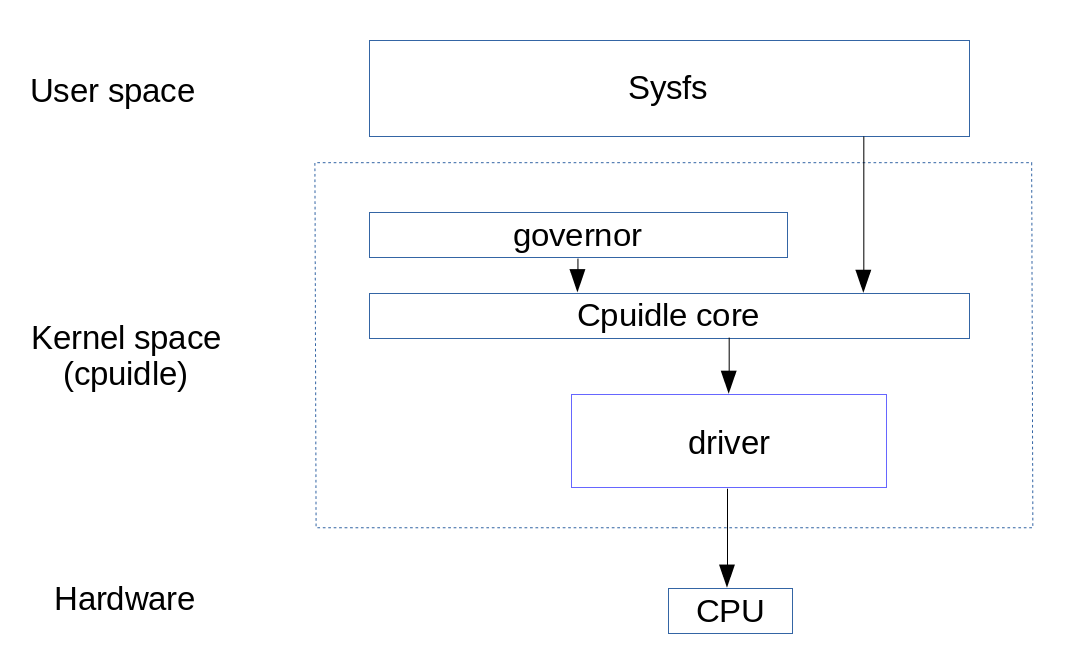
\includegraphics[scale=0.45]{cpuidle1}}
\caption{Общая схема подсистемы cpuidle}
\end{figure}

Сpuidle core включает в себя списки всех зарегистрированных driver и governor, и обнаруженых устройств(CPU), которые описываются структурой device.

Сpuidle core имеет обработчик idle (простоя), \texttt{cpuidle\_idle\_call()}, который будет использоваться каждым отдельным процессором в неактивном состоянии. Перед тем как войти в состояние сна, governor выбирает оптимальное состояние. А затем cpuidle вызывает точку входа для этого конкретного состояния в driver. При возвращении из этого состояния существует необязательный обратный вызов governor для сбора информации о действии этого CPU в состоянии сна.

Число и тип состояний сна могут меняться динамически в зависимости от конкретного состояния данной системы, например от батареи или переменного напряжения. Такое уведомление об изменении состояния системы переходит к driver, который будет вызывать \texttt{cpuidle\_force\_redetect()} в ядре cpuidle. Это приводит к временному удалению обработчика idle, а также к повторному обнаружению driver idle состояния, после чего повторно инициализируется состояние governor, чтобы принять к сведению это изменение.

Чтобы убедиться в том, что мы не запираем обычную процедуру простоя вход/выход и чтобы безопасно изменить governor/driver во время выполнения, используется \texttt{cpu\_idle\_wait} . Обратите внимание, что изменение driver/governor является нераспространенным событием, которое не будет учитывать производительность.

Следует ли cpuidle поддерживать один driver и один governor для всей системы, или же они должны быть для каждого CPU? С учетом простоты реализации governor и driver на программном уровне, в отличие от аппаратного, было решено создать единый driver и governor на программном уровне.

Даже несмотря на то, что переключение между governor и driver может привести к неправильному использованию конечным пользователем, cpuidle поддерживает переключение времени выполнения governor или driver, главным образом, чтобы помочь разработчикам и тестерам cpuidle. В будущем это переключение driver и governor может быть отключено по умолчанию, чтобы избежать неправильного использования.

\subsection{Интерфейс driver}

driver --- архитекурнозависимый элемент подсистемы cpuidle, реализующий перевод вычислительного ядра в состояние сна. В ОС Эльбрус реализацией этой структуры является \texttt{e2k\_driver\_idle}, который вы можете увидеть на рис.

\begin{figure}[h]
\center{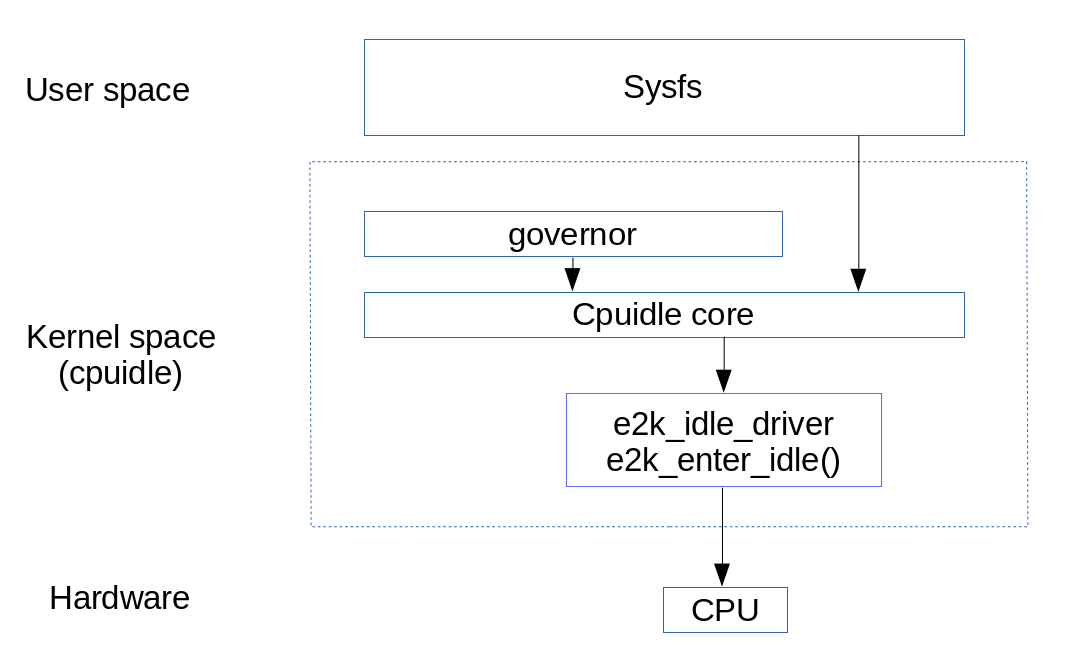
\includegraphics[scale=0.45]{cpuidle4}}
\caption{Общая схема подсистемы cpuidle}
\end{figure}

\texttt{cpuidle\_register\_driver} использует структуру, определяющую интерфейс драйвера cpuidle:
\lstinputlisting{driver.c}
init() --- обратный вызов, вызываемый cpuidle для инициализации каждого устройства в системе с данным driver.

exit() вызывается для выхода из конкретного driver для каждого устройства. Обратный вызов redetect() используется для повторного обнаружения состояний устройства, определенных изменений состояния системы.

При init() driver должен инициализировать все состояния конкретного устройства и обработать общее количество состояний для этого устройства.

Параметры перевода описываются структурой \texttt{cpuidle\_state}:

\lstinputlisting{state.c}

enter() --- это обратный вызов, используемый для непосредственного перевода ядра процессора в состояние сна. \texttt{exit\_latency} и \texttt{power\_usage} являются характеристиками состояния простоя. flags отмечают универсальные возможности и ошибки состояния бездействия. usage является счетчиком времени, в течение которого вызывается состояние сна, а \\time --- время затраченное на это состояние.

\texttt{cpuidle\_register\_driver()} и \texttt{cpuidle\_unregister\_driver()} используются для регистрации и отмены регистрации (соответственно) driver с cpuidle.

\texttt{cpuidle\_force\_detect()} используется driver для того, чтобы заставить cpuidle core повторно обнаружить все состояния устройств (например, после изменения состояния системы).

\subsection{Интерфейс governour}

Как было указано выше governor --- элемент подсистемы cpuidle, определяющий политику перевода вычислительного ядра в оптимальное состояние сна. Ниже показана его структура.

\lstinputlisting{governour.c}

init() --- обратный вызов, вызванный cpuidle, для инициализации каждого governour с устройством (CPU). exit() вызывается для выхода устройства из этого governour.

scan() вызывается при повторном обнаружении состояний устройства. Это дает governour возможность отметить изменения в states во время повторного обнаружения driver.

select() вызывается перед каждым вхождением устройства в состояние сна, чтобы governour мог сделать выбор состояния для вызова idle. reflect() вызывается после выхода из idle, чтобы governour мог захватить информацию о ядре находившемся в этом состоянии. Обратите внимание, что время, затраченное в функции reflect() governor, находится в критическом пути (при выходе из idle, до начала работы) и, следовательно, должно быть быстрым.

\texttt{cpuidle\_register\_governor()}  и \texttt{cpuidle\_unregister\_governor()} используются для регистрации и отмены регистрации (соответственно) governour с cpuidle.

\texttt{cpuidle\_get\_bm\_activity()} получает информацию о деятельности bm, которая может использоваться governour во время процедуры select.

\subsubsection{Реализации}

На данный момент существуют две реализации governor.

\begin{figure}[h]
\center{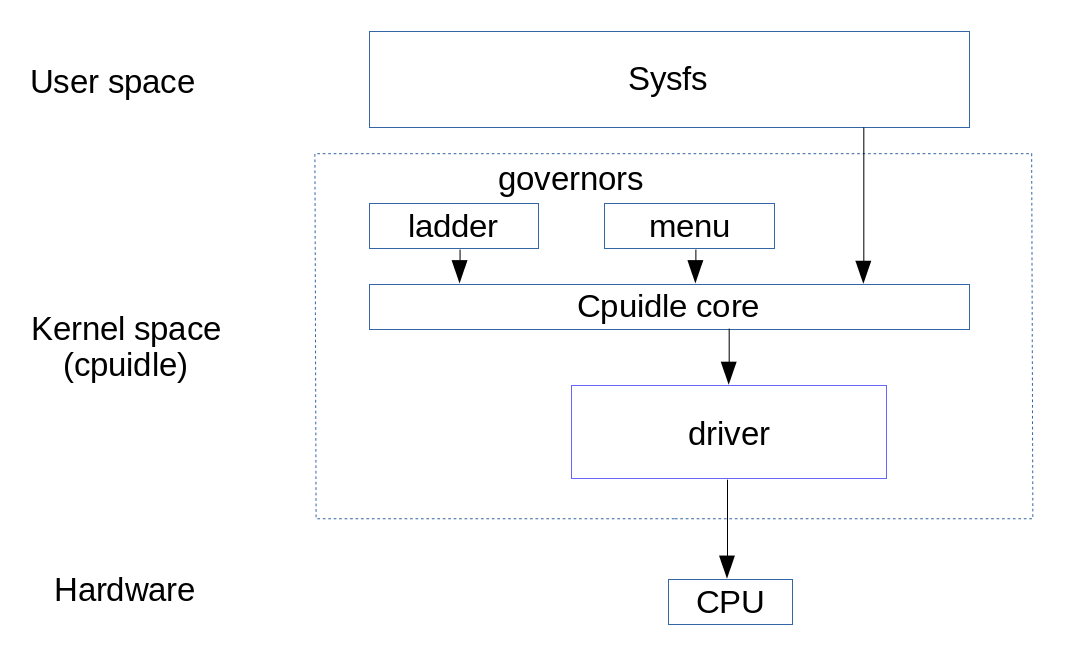
\includegraphics[scale=0.45]{cpuidle2}}
\caption{Реализации governor на общей схеме --- menu и ladder}
\end{figure}

Governor ladder принимает поэтапный подход к выбору состояния сна. Несмотря на то что, эта политка хорошо работает на ядрах процессора с периодическими тактами, она будет плохо себя вести на бестактных (непериодические такты) ядрах. Ядро может оставаться в состоянии сна долгое время без периодических тактов, и у ядра не будет возможности перейти в более глубокий сон

В настоящее время ведется работа над новым governor, который называется menu. Governor menu смотрит на различные параметры, такие как ожидаемое время сна, требования к задержке, предыдущее состояние сна и т. д. Этот governor стремится получить максимальные преимущества, не влияющие на производительность.

\subsubsection{Алгоритм выбора состояния сна}

Выбор оптимального состояния сна зависит от статистики интервалов простоя и загруженности процессора. Оптимальным выбором будем считать состояние, переход в которое не влияет на среднюю производительность операционной системы при заданной загрузке вычислительного комплекса процессами пользователя.
Алгоритм выбора состояния сна, используемый в Linux, основан на анализе четырех
факторов:

\begin{enumerate}
\item duration --- предсказание времени нахождения процессорного ядра в состоянии простоя;
\item correction --- коэффициент поправки предсказания, вычисленный на основе статистики прихода внешних прерываний;
\item latency --- значение времени выхода из состояния сна;
\item \texttt{latency\_mutliplier} --- множитель для значения latency рассчитанный с использованием средней загруженности процессорного ядра.
\end{enumerate}


Для принятия решения алгоритм в цикле рассматривает все состояния сна, начиная с
С3, на каждой итерации проверяя условие:
((latency * \texttt{latency\_mutiplier}) < (duration * correction)).

Если условие справедливо, то выполняется выход из цикла, и управление передается
драйверу PMC, который переводит процессор в выбранное состояние сна.


Заданные в неравенстве величины вычисляются следующим образом. Значение
duration рассчитывается исходя из интервала времени, на которое установлен таймеристочник внешних прерываний для планировщика процессов [7]. Это оптимистичное
предсказание времени нахождения процессорного ядра в состоянии простоя. Для того
чтобы сделать его более реальным, на основе статистики прихода внешних прерываний
рассчитывается коэффициент correction как скользящее среднее от отношения фактического значения времени сна к оптимистической оценке, вычисленного при предыдущем
простое. Если на предыдущем шаге простой продлился 50\% от оптимистической оценки,
то при вычислении скользящего среднего будет использован коэффициент 0,5. Значение
времени выхода из состояния сна latency является константой, которая задается при инициализации драйвера PMC и фиксирована для каждого аппаратно-поддержанного состояния сна. Множитель \texttt{latency\_multiplier} рассчитывается исходя из текущего состояния
средней загруженности процессорного ядра \texttt{load\_average} согласно эвристическому прави-
лу:
\texttt{latency\_multiplier} = (\texttt{load\_average} * 10) + (\texttt{num\_iowaiters} * 5),
где \texttt{num\_iowaiters} – количество процессов, ожидающих на данном процессорном ядре завершения обмена с устройством IO.
Описанный алгоритм является адаптивным и способен выбирать состояние глубоко-
го сна при слабой нагрузке вычислительного комплекса, минимизируя количество пере-
ключений в одно из состояний сна при высокой нагрузке.

\subsection{Device}
Структура содержит информацию о количестве состояний бездействия, которые поддерживаются каждым процессором, информацию о каждом из этих состояний (в массиве ) а также о состоянии этого устройства (CPU).
\lstinputlisting{device.c}

\subsection{Пользовательский интерфейс sysfs}

Пользовательский интерфейс состоит из двух интерфейсов: интерфейс управления и интерфейс мониторинга.

\begin{figure}[h]
\center{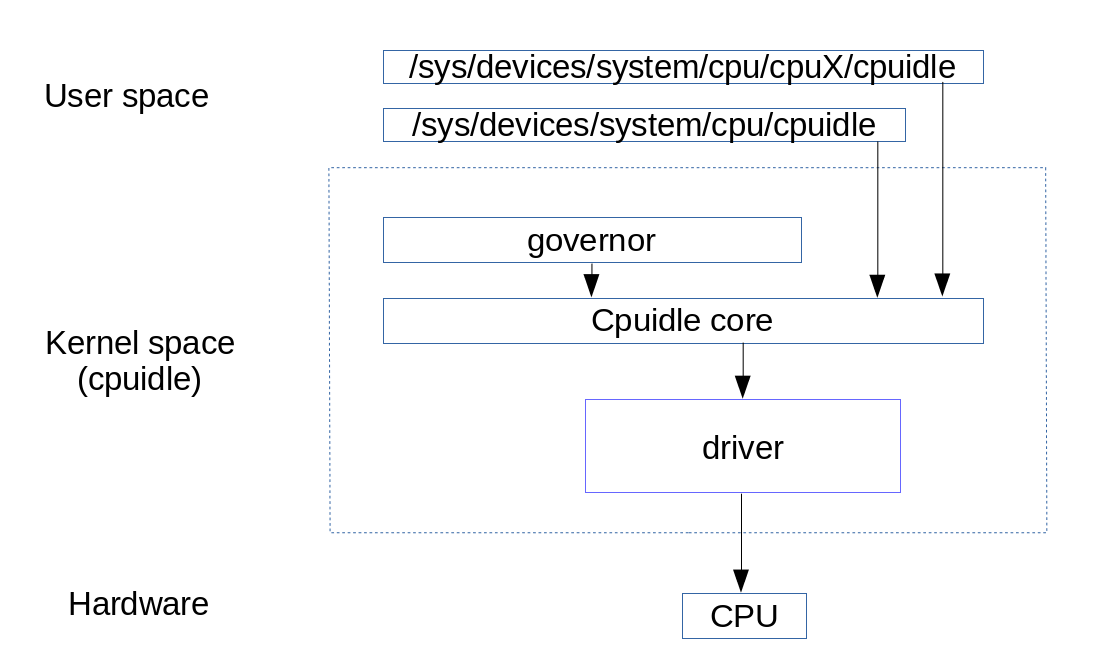
\includegraphics[scale=0.45]{cpuidle3}}
\caption{Общая схема подсистемы cpuidle}
\end{figure}

Следующая информация находится в /sys/devices/system/cpu/cpuidle/.

\texttt{available\_drivers} — файл только для чтения, в котором перечислены все драйверы, успешно зарегистрированные в cpuidle.

\texttt{current\_driver} — файл для чтения и записи, содержащий текущий активный cpuidle driver. Перезаписав значение этого файла на другое из списка доступных driver, меняется driver подсистемы cpuidle.

\texttt{available\_governors} является файлом только для чтения, в котором перечислены все governor, успешно зарегистрированные в cpuidle.

\texttt{current\_governor} — это файл для чтения и записи, содержащий текущий активный cpuidle governor. Перезаписав значение этого файла на другое из списка доступных governor, меняется governor подсистемы cpuidle.

Примечание для всех процессоров, в системе может быть только один governor и один driver.

Следующая информация находится в /sys/devices/system/cpu/cpuX/cpuidle/ где X --- номер ядра.

Для каждого состояния idle, поддерживаемого текущим драйвером, можно увидеть следующую информацию только для чтения под sysfs:

stateY/usage --- число случаев, когда это состояние idle было введено с момента init или redetect.

stateY/time --- время, затраченное на это состояние простоя в микросекундах. 

stateY/latency --- задержка пробуждения для данного состояния.

stateY/power --- типичная потребляемая мощность при входе устройства в это состояние в МВт.


\newpage
\section{Тестирование}
Тестирование проводилось на машинах e401, e801. Запускался тест \texttt{cpuidle\_menu\_tc\_test.sh}. Тест включает модуль cpuidle, меняет governor на ladder и отрабатывает в течение 30 секунд. После работы теста снимаются значения количества вхождений во все три состояния сна с каждого ядра и выводятся на экран. А также изменяется governor на rt, который не переводит ядра в состояния сна.

\begin{figure}[h]
\center{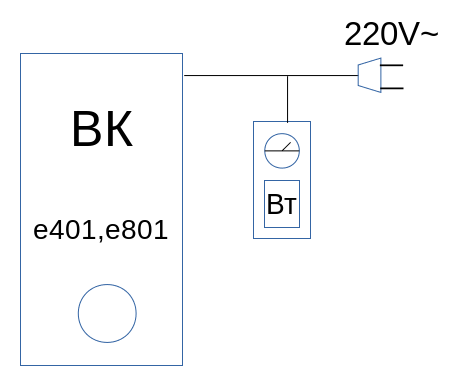
\includegraphics[scale=0.45]{stend}}
\caption{Схема стенда}
\end{figure}

Как видно из результата теста, в состоянии простоя подсистема cpuidle переводит ядра, в основном, в состояние C3. В это же самое время снимались показания с провода питания ВК подключенного к 220V\textasciitilde. В режиме простоя, до включения теста, энергопотребление машины e401 составляло 50.6 Вт, а машины e801 --- 70.4 Вт. Во время работы теста энергопотребление машин составляло 41.8 Вт и 48.4 Вт.

\newpage
\section{Результаты}

\begin{itemize}
\item Реализован алгоритм перевода вычислительного ядра в состояние глубокого сна
\item Алгоритм встроен в подсистему cpuidle
\item Осуществлена возможность управления через интерфейс sysfs
\item При включении соответствующего модуля наблюдается уменьшение энергопотребления ВК e401 на 17\% в состоянии простоя 
\end{itemize}


\newpage

\addcontentsline{toc}{section}{Список литературы}

\begin{thebibliography}{9} 

\bibitem{acpi} Advanced Configuration and Power Interface Specification, Hewlett-Packard Corporation, Intel Corporation, Microsoft Corporation, Phoenix Technologies Ltd, Toshiba Corporation, Revision 4.0a, April 5, 2010.

\bibitem{cpuidle} Venkatesh Pallipadi, Shaohua Li, Adam Belay. «cpuidle – Do nothing, efficiently …», Proceedings of the Linux Symposium 2007, Volume Two, p. 119.

\bibitem{kravc1} Управление энергопотреблением процессорных ядер из операционной системы для прототипа вычислительного комплекса на базе микропроцессоров семейства «Эльбрус», В.С. Волин, Е.М. Кравцунов, д.т.н., проф. С.В. Семенихин, д.т.н. В.М. Фельдман, С.А. Черепанов.

\bibitem{kravc2} Кравцунов Е.М. Пути реализации стандарта ACPI 4.0 (Advanced Configuration and
Power Interface Specification) для многопроцессорных вычислительных комплексов на базе
процессоров «Эльбрус-E2S». – Материалы конференции молодых ученых и специалистов
«Информационные технологии в автоматизированных системах управления специального
назначения», ФГУП НИИАА, 6-7 сентября 2011 г.

\bibitem{tick} Suresh Siddha, Venkatesh Pallipadi, Arjan Van De Ven. Getting Maximum Mileage out
of Tickless. Proceedings of the Linux Symposium 2007, Volume Two, p. 201.

\end{thebibliography}


\end{document}




